\chapter{Method}
\label{chap:Method}
\section{System Overview}
\label{sec:system_overview}

\begin{figure}[htbp]
  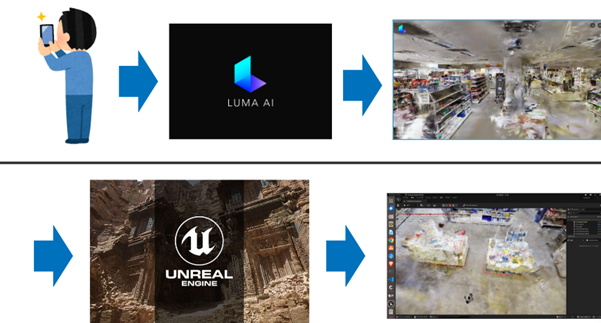
\includegraphics[scale=0.9]{./Figure/画像16.png}
  \caption{Illustration of you writing the master thesis}
  \label{fig:itai}
\end{figure}
\singlespacing
Our research encompasses the development of a three-dimensional, photorealistic environment, culminating in the comprehensive assessment of the Turtlebot3 robot's operational efficacy within this milieu (as elucidated in Figure 3.1). The initial phase entails capturing a video in a verisimilitudinous setting utilizing either an iPhone or an Android smartphone, both equipped with a monocular camera. Post-capture, this footage is uploaded to the advanced Luma AI platform for intricate processing, yielding a three-dimensional, photorealistic environment accompanied by detailed point cloud data. Subsequently, these components are integrated into the Unreal Engine 5 (UE5), facilitating the simulation of a real-world-esque, three-dimensional, photorealistic virtual habitat. Within this UE5 framework, the Turtlebot3 robot conducts a series of simultaneous photographic captures in both the virtual and the actual environments, enabling a holistic evaluation and nuanced analysis of its operational performance in both simulated and tangible real-world scenarios. This comprehensive assessment yields invaluable insights into the robot's functional prowess and its potential applicability across diverse environmental contexts.
\singlespacing
\begin{figure}[htbp]
  \centering
  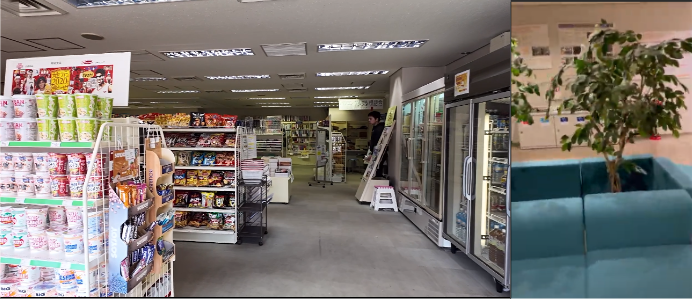
\includegraphics[scale=0.6]{./Figure/画像24.png}
  
  \caption{two real-world environments}
  \label{fig:two real-world environments}
\end{figure}
\section{Video for 3D virtual enviroments}
\label{sec:video for 3D virtual enviroments}
\singlespacing
We recreated two real-world environments as 3D virtual environments using a smartphone camera and a DJI Pocket 2. The environments include a convenience store kiosk, a university educational facility research building, and a laboratory located within the University of Aizu. Our goal was to capture the unique characteristics of each location. The environments include a convenience store kiosk, a university educational facility research building, and a laboratory located within the University of Aizu. Filming took approximately 30 minutes, and select images from each location are shown in \ref{fig:two real-world environments}.
\singlespacing
The images were captured using the iPhone 12 Pro camera and the DJI Pocket 2. The iPhone 12 Pro has three 12MP lenses with different features: ultra-wide angle, wide-angle, and telephoto lenses. The DJI Pocket 2 is a high-performance camera with a compact size and 3-axis stabilization, supporting a variety of video resolutions and modes. With these cameras, high-quality video of three real-world environments was successfully captured.



\section{Video Processing Using Luma AI}
\label{sec:Video Processing Using Luma AI}
\singlespacing
To capture a video and generate a virtual 3D space using LumaAI's NeRF technology, follow these steps:
\singlespacing
First, use your smartphone camera to record the desired environment from multiple angles.  This will provide NeRF with the necessary information to create detailed 3D models. To capture a complete picture of the environment, it is recommended to shoot in slow and steady motions.
\singlespacing
Afterwards, upload the video data to LumaAI's NeRF system, which uses deep learning to analyze the shape and position of objects, lighting conditions, and other factors from each frame in the video to reconstruct a 3D scene.
\singlespacing
After completing the process, LumaAI's NeRF generates a detailed 3D model of the captured environment. This model enables users to observe the scene from different angles, in addition to the original video perspective, allowing for free exploration of the virtual environment.


\begin{figure}[htbp]
  \centering
  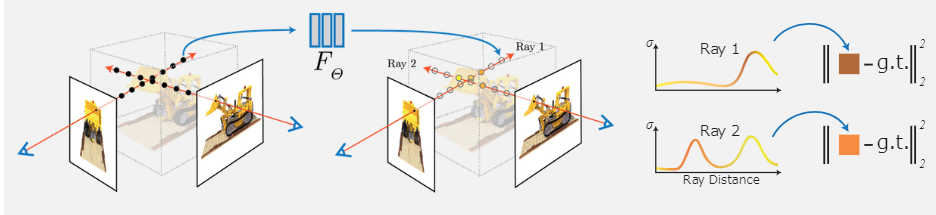
\includegraphics[scale=0.55]{./Figure/画像19.png}
  
  \caption{NeRF synthesizes images by sampling coordinates, processing through an MLP for color and density, and compositing via volume rendering, optimizing by comparing with real images.}
  \label{fig:NeRF synthesizes images}
\end{figure}


\subsection{Neural Radiance Fields (NeRF)}
\label{sec:Neural Radiance Fields (NeRF)}
\singlespacing
Neural Radiance Fields\cite{lin2021inerf}, commonly abbreviated as NeRF, represent a groundbreaking approach in the field of computer vision and 3D reconstruction. This technique, which emerged from the intersection of deep learning and computer graphics, has garnered significant attention for its ability to create highly detailed and photorealistic 3D models from a set of 2D images.
\singlespacing
At its core, NeRF is a novel way to represent 3D scenes. Traditional 3D modeling techniques, like polygon meshes or voxel grids, have limitations in terms of rendering complex details and realistic lighting effects. NeRF addresses these limitations by using a fully connected deep neural network to model the volumetric scene. Essentially, it learns a continuous representation of the scene, mapping spatial coordinates and viewing directions to color and density values. This mapping is achieved through a process called volume rendering, which integrates the contributions of light along a ray passing through the scene(shown in \ref{fig:NeRF synthesizes images}).
\singlespacing
One of the most striking features of NeRF is its ability to synthesize novel views of a scene with high fidelity. Given a set of 2D images taken from different viewpoints, NeRF can interpolate and extrapolate from this data to generate new images from perspectives not originally captured. This is particularly valuable in applications like virtual reality, where immersive experiences depend on realistic and fluid rendering of 3D environments.
The training process of a NeRF model involves optimizing the neural network to minimize the difference between the rendered images and the actual input photographs. This optimization is computationally intensive, as it requires processing thousands of rays through the neural network to accurately capture the light interactions in the scene. However, the results are often stunning, with NeRF models capable of capturing intricate details like reflections, refractions, and complex lighting conditions that are challenging for traditional 3D modeling methods.
\singlespacing
NeRF's applications extend beyond just creating photorealistic renderings. It's also being explored in fields like cultural heritage preservation, where it can be used to create detailed digital replicas of historical artifacts or sites from a limited number of photographs. In robotics and autonomous vehicles, NeRF can assist in creating detailed 3D maps of environments. In the film and entertainment industry, it offers new possibilities for visual effects and virtual production, allowing for seamless integration of virtual and real elements.
\singlespacing
Despite its impressive capabilities, NeRF does have some limitations. The computational resources required for training and rendering are significant, which can be a barrier to real-time applications. Additionally, the quality of the output heavily depends on the quantity and quality of the input images. Scenes with highly dynamic elements or transparent objects still pose challenges for NeRF models.
\singlespacing
In conclusion, Neural Radiance Fields represent a significant advancement in 3D scene representation and rendering. By leveraging the power of deep learning, NeRF offers a way to create highly detailed and realistic 3D models from ordinary photographs. Its potential applications are vast, spanning various industries, and it continues to be an active area of research, with ongoing efforts to overcome its current limitations and expand its capabilities.
\singlespacing
\begin{figure}[htbp]
  \centering
  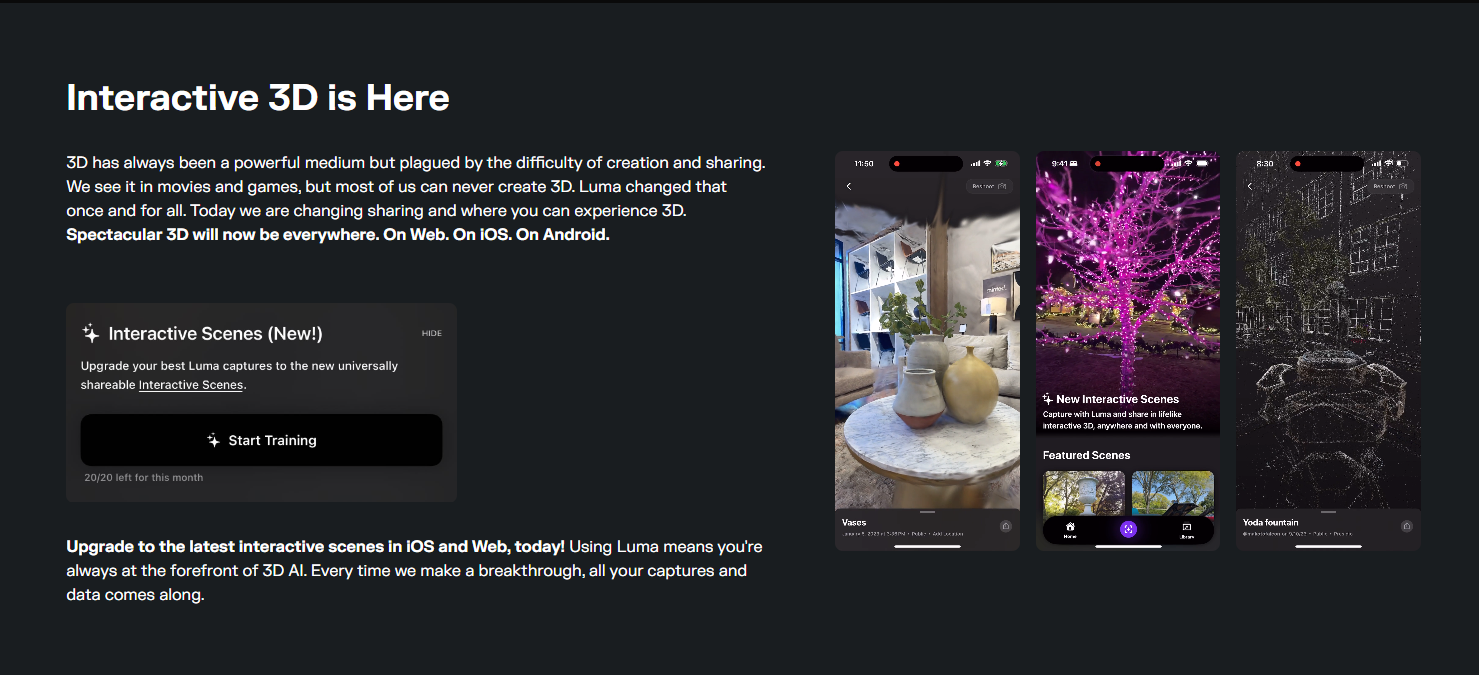
\includegraphics[scale=0.35]{./Figure/画像20.png}
  \caption{Luma AI Platform site}
  \label{fig:Luma AI Platform site}
\end{figure}
\subsection{Luma AI Platform}
\label{sec:Luma AI Platform}
\singlespacing
Luma AI\cite{lumaai} is an innovative scanning application capable of capturing objects in three dimensions. This app stands out for its ability to generate and output precise 3D models, available in both a web version and an iOS version. Users can create 3D models by uploading videos or capturing real objects using a smartphone camera. Notably, Luma AI utilizes NeRF (Neural Radiance Fields) technology, which reconstructs three-dimensional states through machine learning using multiple photographs.
\singlespacing
Delving into the usage of this app, one must first set up an account, followed by capturing the object from various angles through filming or photography. After uploading these videos or photos to Luma AI(see.\ref{fig:Luma AI Platform site}), the AI employs this data to generate a highly detailed 3D model of the targeted object. These models can be converted into various formats such as GLTF, OBJ, or USDZ, offering flexibility in usage. By default, captures are set to private, but options are available to share them publicly with the Luma AI community or with selected individuals
\singlespacing
Moreover, Luma AI is compatible with 3D printers, enhancing its utility for game engine developers and visual effects artists. The app's capabilities include capturing unparalleled photorealism, intricate details, and vivid reflections, making it a vital tool for game developers and VFX artists. These features underscore Luma AI's significance in these fields.
\singlespacing
Regarding pricing, the basic Luma AI toolset is entirely free, with a nominal fee of \$1 per capture when using the API. The Luma AI API is designed to process video walkthroughs of objects or scenes, offering some of the world's finest 3D modeling and reconstruction capabilities to developers at an incredibly affordable rate


\begin{figure}[htbp]
  \centering
  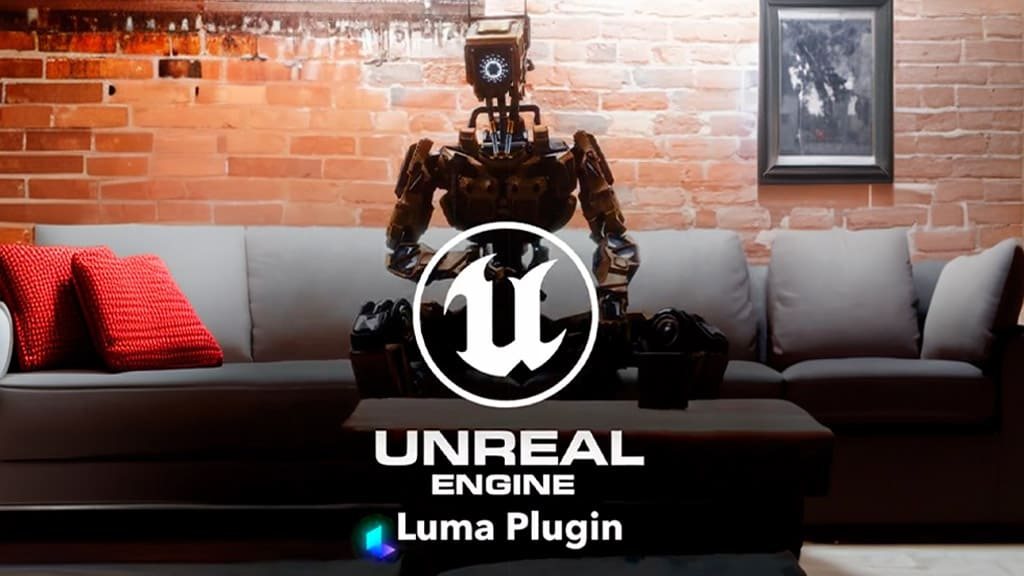
\includegraphics[scale=0.35]{./Figure/画像21.jpg}
  \caption{Unreal Engine 5 and Luma AI integration}
  \label{fig:Unreal Engine 5 and Luma AI integration}
\end{figure}
\begin{figure}[htbp]
  \centering
  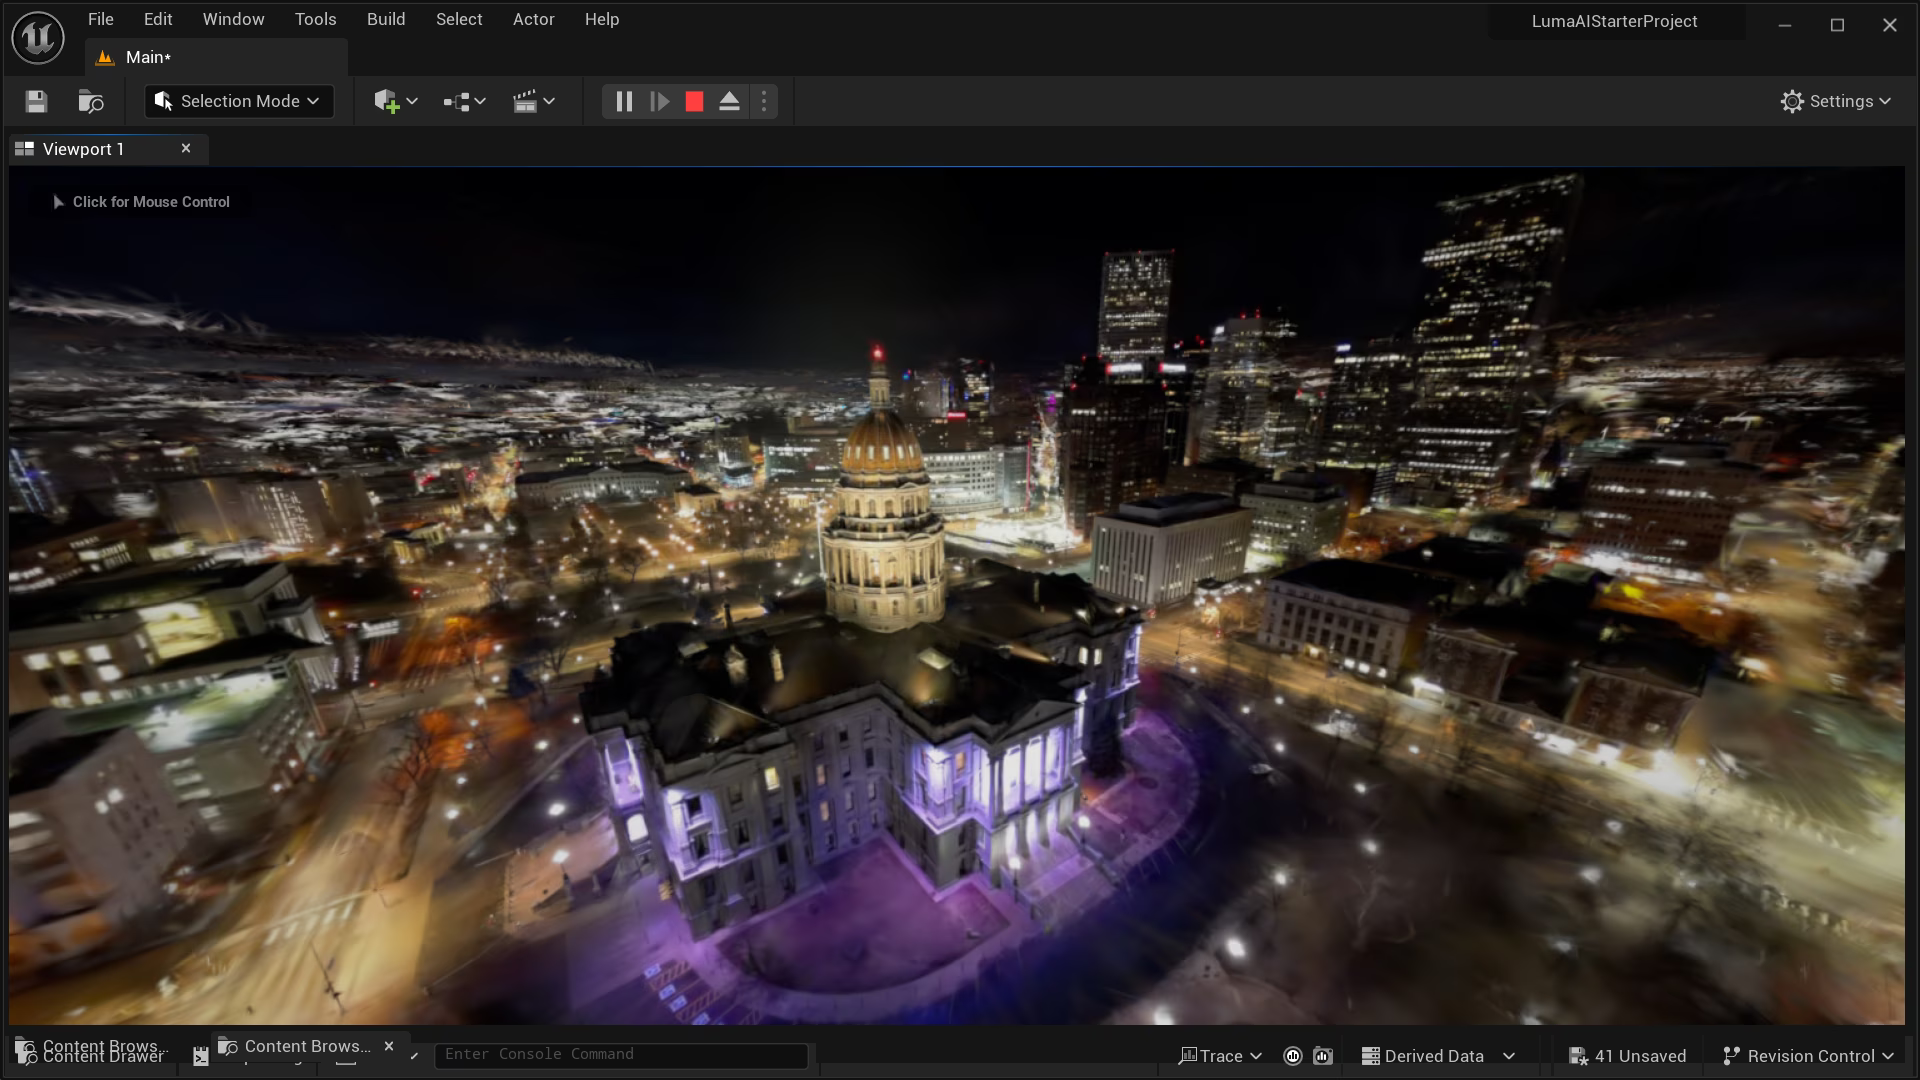
\includegraphics[scale=0.2]{./Figure/ppp.png}
  \caption{Unreal Engine 5 and Luma AI integration presents 3D virtual enviroment in Unreal engine5}
  \label{fig:Unreal Engine 5 and Luma AI integration presents 3D virtual enviroment in Unreal engine5}
\end{figure}

\section{3D Photorealistic Environment in Unreal Engine 5}
\label{sec:3D Photorealistic Environment in Unreal Engine 5}
\singlespacing
The process of integrating Luma AI and Unreal Engine 5 (UE5) is a significant aspect in the realm of advanced computer graphics and AI-driven applications\cite{luma2023unreal}(see Fig.\ref{fig:Unreal Engine 5 and Luma AI integration}, \ref{fig:Unreal Engine 5 and Luma AI integration presents 3D virtual enviroment in Unreal engine5}). It commences by obtaining data processed by Luma AI, usually obtainable for download from the Luma AI website in the .luma format. These .luma files contain the data processed by Luma AI and constitute a pivotal junction of AI processing and graphical rendering.
\singlespacing
The next step is to import the .luma files into UE5. This is done by placing them within Unreal Engine 5's content management system. The data processed by Luma AI is then integrated directly into UE5. This allows users to take advantage of UE5's advanced rendering and simulation capabilities, enhanced by the AI-driven data from Luma AI. This collaboration showcases the synergy between AI processing and real-time rendering, leading to enhanced and lifelike simulations in virtual environments.
\singlespacing
\begin{figure}[htbp]
  \centering
  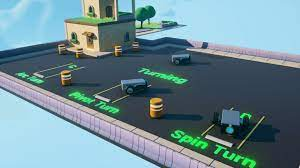
\includegraphics[scale=1]{./Figure/robot_in_unreal_engine.jpg}
  \caption{robot in Unreal engine5}
  \label{fig:robot in Unreal engine5}
\end{figure}
\subsection{Unreal Engine 5}
\label{sec:Unreal Engine 5}
\singlespacing
Unreal Engine 5 (UE5) \cite{unreal2023engine}is a game engine developed by Epic Games. It is the successor to Unreal Engine 4, which was released in 2014. The engine was first announced in March 2018 and was released in early access on May 13, 2021. The engine is designed for use in video games, but it can also be used for other applications such as virtual reality, augmented reality, and architectural visualization. Unreal engine 5 are used in robotics (see Fig.\ref{fig:robot in Unreal engine5})
\singlespacing
At the heart of Unreal Engine 5 lies its revolutionary rendering architecture, designed to deliver photorealistic visuals and dynamic global illumination in real-time. This is primarily facilitated by two core technologies: Nanite and Lumen. Nanite is a virtualized geometry technology that allows artists to create as much geometric detail as the eye can see. This virtualized micropolygon geometry frees creators from polygon budget constraints and the often tedious and time-consuming task of baking details into normal maps. With Nanite, users can import film-quality source art comprising hundreds of millions or billions of polygons directly into Unreal Engine, and it will be streamed and scaled in real time with no loss in quality.
\singlespacing
Lumen, on the other hand, is a fully dynamic global illumination solution that reacts immediately to scene and light changes, accurately simulating the subtle and complex interplays of light and shadow in an environment. With Lumen, artists and designers can create more dynamic scenes, where indirect lighting adapts on the fly to changes to direct lighting or geometry, such as changing the sun's angle with the time of day, turning on a flashlight, or opening an exterior door. This leads to a significant reduction in the time required to tweak lighting scenarios and settings, enabling a more intuitive design process.
\singlespacing
Another major feature of Unreal Engine 5 is its enhanced support for open worlds and large-scale environments. This is achieved through a new World Partition system, which changes how levels are managed and streamed, automatically dividing the world into a grid and streaming the necessary cells. This system makes it easier for teams of any size to collaborate on massive worlds without running into the typical bottlenecks associated with such large-scale projects.
\singlespacing
Unreal Engine 5 also introduces significant improvements in animation and physics. The engine integrates a new animation toolset that facilitates more dynamic and realistic movements and interactions. The advancements in physics simulation, along with the introduction of the Niagara VFX system, allow for more detailed and interactive environments. These features are essential for creating immersive experiences in games and simulations, where realism and responsiveness are key.
\singlespacing
Furthermore, UE5 includes robust audio tools like MetaSounds, a high-performance system that provides complete control over audio DSP graph generation of sound sources, leading to richer, more dynamic auditory environments. This level of control enables sound designers to create more complex and dynamic auditory experiences that can adapt in real time to the game or scene's events.
\singlespacing
In terms of usability, Unreal Engine 5 has been designed with a focus on making it more accessible and user-friendly, without sacrificing the depth and complexity that experienced developers expect. The user interface has been refined, and new features like the UI of Quixel Bridge have been integrated directly into the engine, streamlining the workflow for accessing a vast library of high-quality assets.
\singlespacing
In conclusion, Unreal Engine 5 represents a quantum leap in game engine technology, offering groundbreaking innovations in graphics rendering, world-building, animation, physics, and audio. Its suite of tools and features positions it as a key enabler for the next generation of real-time 3D content, pushing the boundaries of what is possible in game development, film production, architectural visualization, and beyond. Its focus on scalability, performance, and quality makes it a versatile choice for developers and creators aiming to craft experiences that are both visually stunning and deeply immersive.



\begin{figure}[htbp]
  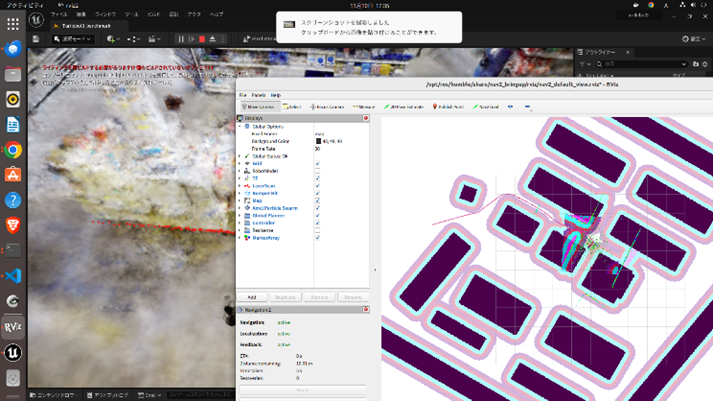
\includegraphics[scale=1.8]{./Figure/画像17.png}
  \caption{We navigated Turtlebot3 by navigation2  in Unreal Engine 5}
  \label{fig:We navigated Turtlebot3 by navigation2  in Unreal Engine 5}
\end{figure}

\section{Deployment of Turtlebot3 Robot in Virtual Environments}
\label{sec:Deployment of Turtlebot3 Robot in Virtual  Environments}
\singlespacing
The deployment of the Turtlebot3, specifically the waffle model, provides an intriguing case study in real and virtual robotic environments. Unreal Engine 5 (UE5) is used as the simulation platform in the virtual environment, and integrating the Turtlebot3 waffle with UE5 is accomplished using rcIUE\cite{rapyuta2023rclue}in conjunction with ROS2 Humble. This configuration enables the utilisation of sophisticated robotic features like Navigation2 and Simultaneous Localization and Mapping (SLAM). UE5's deployment enables thorough testing and enhancement of the robot's abilities through an extensive and lifelike simulation platform, unbound by any physical limitations.
\singlespacing
To operate in the actual environment(see.Fig.\ref{fig:We navigated Turtlebot3 by navigation2  in Unreal Engine 5}), we use the same Turtlebot3 waffle model, which is directed using ROS2 Humble. Directly controlling the robot in a physical setting enables practical implementation and testing, providing valuable insights into its performance and adaptability in real-world scenarios. The transition from virtual to physical environments highlights the versatility of the Turtlebot3 Waffle and its compatibility with ROS2 Humble, demonstrating its potential for diverse applications in the field of robotics.
\singlespacing
\section{Virtual Environment Evaluation}
\label{sec:Virtual Environment Evaluation}
\singlespacing
For the evaluation of our robotic simulation environment, we used Navigation2 to assess operational efficacy in a virtual setting, achieving a high success rate. We also integrated object recognition capabilities using You Only Look Once (YOLO). Specifically, we used a pre-trained YOLOX\cite{ge2021yolox} model. This study focused on recognizing objects in both real and virtual environments, with a particular emphasis on identifying identical objects across these settings. The effectiveness of cross-environment object recognition was quantitatively measured using the F1 score. We conducted a comprehensive analysis comparing the time and resources required to create virtual environments using our approach with those required for other studies such as NeRF2Real\cite{byravan2023nerf2real} and Matterport3D\cite{chang2017matterport3d}. The analysis focused on aspects such as computational efficiency and the need for specialized expertise. This comparison provided valuable insights into the relative performance and efficiency of our approach within the broader context of robotic simulation research.
\singlespacing
The F1 score is calculated as:
\begin{equation}
  precision = \frac{TP}{TP + FP}
\end{equation}
  
\begin{equation}
  recall = \frac{TP}{TP + FN}
\end{equation}

\begin{equation}
  F1-score = 2 \times \frac{precision \times recall}{precision + recall}
\end{equation}
\singlespacing
Here, TP (True Positives) is the count of objects correctly recognized as the same in both real and virtual environments, and FP (False Positives) is the count of objects that are incorrectly recognized as the same. FN (False Negatives) is the count of objects that are actually the same in both environments but were not recognized as such.

\subsection{YoloX}
\label{sec:You Only Look Once(Yolo)X}
\singlespacing
YOLOX\cite{ge2021yolox} represents the cutting-edge in real-time object detection within the realm of deep learning algorithms. As an evolution of the YOLO (You Only Look Once) series, YOLOX distinguishes itself by its ability to detect objects in an image through a singular inference process. This contrasts sharply with traditional object detection systems, which typically require a two-stage process involving region proposal and classification. YOLOX, however, amalgamates these tasks, achieving both simultaneously in one fell swoop.
\singlespacing
\begin{figure}[htbp]
  \centering
  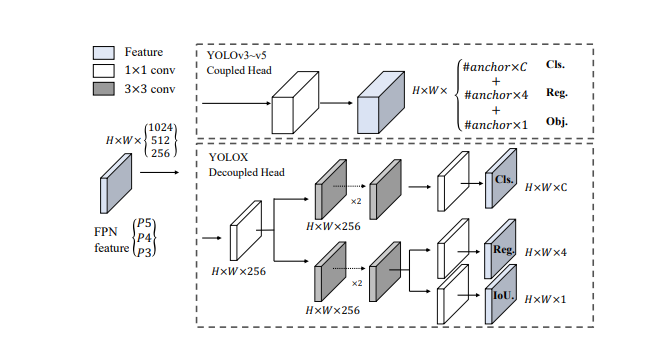
\includegraphics[scale=0.6]{./Figure/画像22.png}
  \caption{Illustration of the difference between YOLOv3 head and the proposed decoupled head.}
  \label{fig: Illustration of the difference between YOLOv3 head and the proposed decoupled head.}
\end{figure}
\singlespacing
The architecture of YOLOX is a tripartite structure, comprising a backbone, a neck, and a head. Each component plays a pivotal role: the backbone extracts features from images, the neck refines these features, and the head is responsible for the final object detection and classification.


\subsubsection{Backbone}
\label{sec:Backbone}
\singlespacing
The backbone typically employs efficient convolutional networks, such as Darknet or CSPDarknet. These networks are adept at extracting salient features from images with high efficiency.

\subsubsection{Neck}
\label{sec:Neck}
\singlespacing
The neck utilizes structures like Feature Pyramid Networks (FPN) or Path Aggregation Networks (PAN) to integrate features across different scales. This integration enhances the detection capabilities for objects of varying sizes, from the diminutive to the substantial.

\subsubsection{Head}
\label{sec:Head}
\singlespacing
In the head segment, bounding box prediction and class classification occur. YOLOX adopts an anchor-free approach, which, compared to traditional anchor-based methods, offers more flexibility and efficiency in object detection.



The core of YOLOX's functionality can be described through its loss function, which is a combination of coordinate loss, objectness loss, and class classification loss.
\singlespacing
\begin{align}
\text{Loss Function} = & \ \lambda_{\text{coord}} \times \text{Coordinate Loss} \nonumber \\
                      & + \lambda_{\text{obj}} \times \text{Objectness Loss} \nonumber \\
                      & + \lambda_{\text{cls}} \times \text{Class Classification Loss}
\label{equ:Loss Function}
\end{align}

Where $\lambda_{\text{coord}}$, $\lambda_{\text{obj}}$, and $\lambda_{\text{cls}}$ are the weights for the respective losses.

\subsubsection{Coordinate Loss}
\singlespacing
Coordinate loss measures the discrepancy between predicted and actual bounding boxes, often using an IoU-based loss.

\subsubsection{Objectness Loss}
\singlespacing
Objectness loss assesses the error in predicting the presence of an object, typically employing binary cross-entropy loss.

\subsubsection{Class Classification Loss}
\singlespacing
Class classification loss evaluates the error between predicted and actual classes, using cross-entropy loss.
\singlespacing
YOLOX is a powerful tool in real-time object detection, offering a blend of speed and accuracy. Its ongoing development is expected to continue pushing the boundaries in the field of computer vision.

